\documentclass[jou,apacite]{apa6}

\title{Book Analysis: Harnessing Complexity}
\shorttitle{Book Analysis}

\author{Steve Mazza}
\affiliation{Naval Postgraduate School}

\abstract{Throughout this book the authors develop and present a framework for coming to terms with complexity that we are likely to find in systems with which we interact every day.  Banking, the global commerce that results in affordable goods, the Internet, and our relationships at work are all examples of complex adaptive systems.  The framework that they present is intended to help us better understand the complexities inherent in these systems and also to assist us in harnessing this complexity in order to maximize our gain.  It is not an attempt to game the system, rather to help us better understand the interactions among the moving parts and to apply that understanding to our benefit.}


\rightheader{Book Analysis}
\leftheader{Steve Mazza}

\begin{document}
\maketitle    
                        
\section{Introduction}
Throughout this book the authors develop and present a framework for coming to terms with complexity that we are likely to find in systems with which we interact every day.  Banking, the global commerce that results in affordable goods, the Internet, and our relationships at work are all examples of complex adaptive systems.

The framework that they present is intended to help us better understand the complexities inherent in these systems and also to assist us in harnessing this complexity in order to maximize our gain.  It is not an attempt to game the system, rather to help us better understand the interactions among the moving parts and to apply that understanding to our benefit.

What we will show is that the framework presented here assists in relating the principles and attributes of complex adaptive systems to real world complex systems in a way that facilitates the users understanding of those systems to his benefit.

In all cases, information not specifically cited is derived in whole or in part from the primary text, \emph{Harnessing Complexity: Organizational Implications of a Scientific Frontier} by Robert Axelrod and Michael Cohen.

\begin{figure}[htpb]
  \centering
  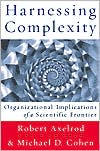
\includegraphics[width=0.35\columnwidth]{images/harnessingComplexity.jpg}
  \caption{Harnessing Complexity, Axelrod \& Cohen}
  \label{fig:hc}
\end{figure}

They begin with an introduction of the terminology and develop ideas connecting these terms to the real world.  They then introduce the mechanisms of variation, interaction, and selection, which are all treated in the context of the presented framework.  We will discuss these in the sections that follow.

The authors provide a summary of how the parts of the framework form a working whole.  While they present this in the conclusion, we find it a provides useful context during the rest of the discussion.
\begin{quote}
  Agents, of a variety of types, use their strengths in patterned interaction, with each other and with artifacts.  Performance measures on the resulting events drive the selection of agents and/or strategies through processes of error-prone copying and recombination, thus changing the frequencies of the types within the system.~\cite[page 154]{Axelrod}
\end{quote}
While this description may seem overly abstract, it is actually a succinct recitation of the framework and makes sense in the context of the ontology presented below.

\section{Background}

There are several central ideas that have guided the development of the framework, which we will briefly introduce.

First, there exists a certain difficulty regarding prediction that is exacerbated by complexity.  The heavy dependence on initial conditions coupled with the highly interactive nature of the moving components in a complex system creates nontrivial difficulty in anticipating its outcome.

Second, the themes supported by models of complexity have application across a variety of disciplines including the physical, biological, and social sciences.  Examples from these domains include microchip design, food networks, and your Facebook account.

Third, the concepts contained within the framework provide us with a mechanism by which we can categorize, anticipate, and better understand consequences that are difficult to predict.

Lastly, the framework is an embodiment of, ``the main mechanisms and design principles that we identify from complex systems research.''~\cite[page 2]{Axelrod}  That is, it builds on current research in complex systems in a way that extends its accessibility so other scientific endeavors as well as the mundane\footnote{We are referring to routine complex systems that we may tend to take for granted such as two day Amazon package delivery}.

\subsection{Applying the Framework}

The authors introduce three questions that will help guide the user in applying the framework to complex adaptive systems.  These questions will assist the user in focusing his attention on specific parts of the framework as they apply to real world systems.  The first question is, ``What is the right balance between variety and uniformity?''  Facilitating an optimal solution often means carefully balancing exploration and exploitation.  In this context, exploration equates to the
introduction of more variety, as it leads to increasingly diverse combinations.  Exploitation equates to uniformity, getting the maximum yield from the existing resources, actors, strategies, and environmental conditions.

``Who should interact with what, and when?''  This is a strategy and interaction pattern question.  What environmental conditions should be established or adjusted in order to ensure the right interactions among the right agents at the right time?

The third and final question to guide the user is, ``Which agents or strategies should be copied and which should be destroyed?''  This question gets at measures of success, attribution of credit, and evolution.  To couch the question in slightly crass terms, who has earned the right to reproduce?

\subsection{Coming To Terms}

The authors introduce key terms and develop definitions for the following, which we will present and briefly comment on.  The identification of these key terms serves as the basis for effectively communicating the ideas about the framework. They create a meaningful ontology that we can use to extend the ideas presented in this book to the complex adaptive systems we encounter every day.

\subsubsection{Agent}
The agent is the component of the model responsible for purposeful action.  Agents interact with their environment in meaningful ways and, while frequently thought of as people, can be any entity capable of initiating action such as businesses, countries, or computer programs.  In many models, agents play a central and prominent role.  The agent is often the benefactor of change or optimization in the model and frequently (but not always) the motivation for creating the model in the first place.

\subsubsection{Strategy}
The strategy is the set of rules that an agent applies in response to changing environmental conditions.  In a model, these are the rules that we adjust in order to affect a desired outcome.  In real life, this is the set of heuristics and actions we apply in an attempt to have things go our way.  We may chose to cooperate or compete or to be patient or aggressive.  But we chose our strategy based on assumptions of achieving a desired outcome.  The authors make note of how strategies can
be adapted over time based on the achievement (or lack of achievement) of the agent's goals.

\subsubsection{Measure of Success}
How an agent sees the acquisition of or progress toward desired outcomes is gauged by measures of success.  These can be any metrics that the agent can observe within the environment.  They are often used to inform changes to strategy.  As an example, suppose you are trying to get some help on a project at work.  You have asked nicely several times to no good effect.  The measure of success is the level of assistance you have been able to get on the project.  If it is too low, you may alter
your strategy by involving a supervisor.

\subsubsection{Copying}
This refers to the duplication of effort by actors usually through the transfer of knowledge or information about how to affect an outcome.   This transfer of knowledge can be exact like in the case of a computer or error prone like in the case of the training of a newly hired employee.  Error in copying is sometimes beneficial because it introduces a randomness that adds to the diversity of the population, or group of agents.

\subsubsection{Population}
A population is a collection of agents or groups of agents and constitutes the entirety of those agents either as a whole or by some more narrowly defined characteristic.  It is also possible to think about populations of strategies.

\subsubsection{Type}
A type is a characteristic or attribute that defines a segment of the whole population.

\subsubsection{Variation}
This is the diversity among types in a population and often results from copying errors, as in evolution.  In many circumstances too much variety can lead to low copy rates (e.g., low birth rate).  For example if there are not a sufficient number of suitable mates then a particular population type may dwindle.  But more often, variation leads to much more interesting combinations and consequences.  After all, variety is the spice of life!

\subsubsection{Interaction Patterns}
These are the ways in which agents are likely to interact.  They are influenced by rules as well as other environmental factors.  Consider the coffee shop that you frequent on your way to work.  Your choice to stop there is shaped not only by the courteous staff and good coffee but also by the topography, roads, traffic lights, and other commuters between your home and work.  It is shaped by your desire for coffee, which drives this interaction pattern. And it is shaped by the fact that
everyone at work makes lousy coffee.

\subsubsection{Artifacts}
These are used by agents and have properties similar to agents.  They may also have ``affordances'' that evoke specific behaviors from agents. A guitar has a shape that beckons the user to pick it up, hold it, and strum the strings.  The form of the instrument encourages its use.

\subsubsection{System}
This refers to the entire environment including the agents, strategies, artifacts, and pertinent environmental factors.  Changes in policy or practice as well as brand new creations all require work at a system level.

\subsubsection{Complex}
The authors describe complexity best as, ``[A] system is complex when there are strong interactions among its elements, so that current events heavily influence the probabilities of many kinds of later events.''~\cite[page 7]{Axelrod}  Pay attention to the fact that complexity does not necessarily mean there are a lot of moving parts.  But that the parts that move have strong interactions.

\subsubsection{Selection}
This can be thought of as the way in which variety finds favor (or benefit).  Variation yields new combinations, sometimes by accident, occasionally resulting in a stronger or more capable agent.  If selection favors a particular agent then that agent will become more prolific.  The opposite is also true.

\subsubsection{Adaptation}
This is the result of a favorable selection process.  It can be thought of as marking an event that ratchets forward the progress of an agent toward some desirable end.

\subsubsection{Complex Adaptive System}
Any system with a population that seeks to adapt can be called a complex adaptive system, given that the system itself is sufficiently complex.

\subsubsection{Co-evolutionary Process}
This is the result of multiple populations of agents adapting to each other.  The idea is that any one population of agents would, itself, constitute a complete system, along with artifacts, strategies, and other appropriate environmental factors.

\subsubsection{Harnessing Complexity}
``[D]eliberately changing the structure of a system in order to increase some measure of performance, and to do so by exploiting an understanding that the system itself is complex.''~\cite[page 9]{Axelrod}

\subsubsection{Emergent Properties}
These are attributes of a system that are not individually accounted for by any of the constituent parts.  Emergence does not always occur.  But when it does, it imparts a value to the system beyond the component parts.

\subsubsection{Complicated}
Versus complex (see previous term), a system is complicated if it simply has many moving parts.

\subsubsection{Attribution of Credit}
This describes the process by which the winning and losing strategies are determined.

\subsubsection{Designer}
The introduction of new strategies and artifacts is done by the designer.

\subsubsection{Policy Makers}
By increasing rewards for some outcome or altering some pattern of interaction, policy makers alter the consequences of available strategies with malice of forethought.

% The following are the central concepts that do most of the work in the Complex Adaptive Systems approach presented by the authors.
% \begin{itemize}
  % \item Strategy, a conditional action pattern that indicates what to do in which circumstances.
  % \item Artifact, a material resource that has definite location and can respond to the actions of agents.
  % \item Agent, a collection of properties (especially location), strategies, and capabilities for interacting with artifacts and other agents.
  % \item Population, a collection of agents, or, in some situations, collections of strategies.
  % \item System, a larger collection, including one or more populations of agents and possibly also artifacts.
  % \item Type, all the agents (or strategies) in a population that have some characteristic in common.
  % \item Variety, the diversity of types within a population or system.
  % \item Interaction pattern, the recurring regularities of contact among types within a system.
  % \item Space (physical), the location in geographical space and time of agents and artifacts.
  % \item Space (conceptual), the ``location'' in a set of categories structured so that ``nearby'' agents will tend to interact.
  % \item Selection, processes that lead to an increase or decrease in the frequency of various types of agents or strategies.
  % \item Success criteria or performance measure, a ``score'' used by an agent or designer in attrubuting credit in the selection of relatively successful (or unsuccessful) strategies or agents.
% \end{itemize}

\section{Energizing the Framework}
So now that we have established our ontology and set up our framework, it is time to put it to some good use.  In doing so, we want to consider three key influencers that have the greatest impact on the outcomes of the system.

\begin{figure}[htpb]
  \centering
  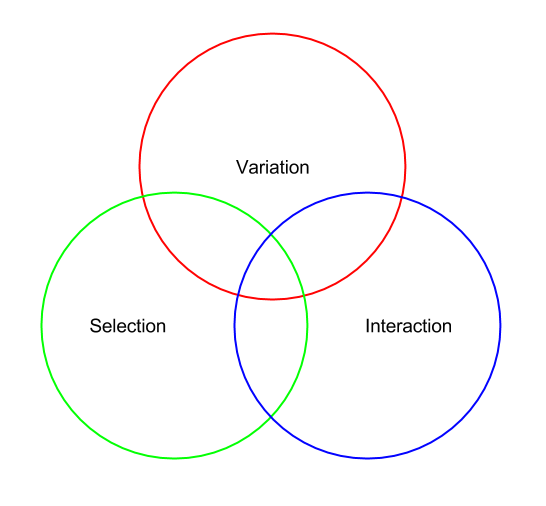
\includegraphics[width=0.9\columnwidth]{images/vis.png}
  \caption{Key influencers of complex adaptive systems.}
  \label{fig:vis}
\end{figure}

\subsection{Variation}
``Variation provides the raw material for adaptation.''~\cite[page 32]{Axelrod}  The amount and type of variation provides the basis for resolving the distinction between exploration and exploitation in a system.  Greater variation maps to exploration, as agents are replicated with error and recombine in often unanticipated ways.  

Whether to encourage variation depends on the amount of resources currently available and the success with which the current population is using it.  Another consideration is the population size.  It is often the case that for a population to be successful (for a population to successfully exploit its environment) there must first exist a sufficient population size, without which success is significantly less likely.

Variation is the result of copying with error and recombination.  Copying with error happens in many complex adaptive systems and the authors select the example of training new employees in a workforce.  Transfer of information (e.g., policies, procedures, or organizational data) among people is necessarily lossy as exemplified in the childhood game where you sit in a circle and pass a short phrase from one to another until it makes its way back to where it started.  Invariably, the
information is badly corrupted by that point.

\subsection{Interaction}
The key question, introduced previously, is, ``What should interact with what, and when?''~\cite[page 62]{Axelrod}  This is a heavily laden question that gets at the heart of how agents are exposed to each other, artifacts, and other pertinent elements in their environment.  Factors influencing interaction may be spacial (physical or logical) temporal, or just good (mis)fortune.

There must exist some proximal relativity among agents for interaction to occur.  Our commute to work brings us in contact with the same coffee shop, the same bus driver we get stuck behind, and the same roads (physical infrastructure, or artifacts).  These interactions afford us opportunities that we would not otherwise have by virtue of our proximity to other actors and artifacts.  It also necessarily precludes other interactions.

Another key concept in interaction is activation, or the key sequence of events that leads to interaction.  The distinction between proximity and activation is important because they often work in concert.  And in order to properly harness the power in a complex system it is critical to distinguish between spatial and temporal causes (i.e., between proximity and activation).

An easy example of activation is the ``externally clocked'' timing of Conway's Game of Life.  As with many cellular automata, evolution occurs simultaneously for each agent on every clock tick.  Activation, therefore, is concurrent for each eligible agent.  This is an example of external activation.  

Activation may, however, be internal.  In these cases, agents may derive some benefit from a high level of fitness by being eligible for more frequent activation or possibly activation in some preferential order.  In many biological systems, stronger agents are able to feed, mate, and find shelter with preference over weaker agents.

An omniscient designer might alter interactions to affect some perceived benefit.  Methods of altering interaction patterns include constructing and removing barriers.  Consider a detour due to roadwork that causes you to seek out a different coffee shop on your way to work.  This might also remove the school bus as an obstacle but may present different opportunities for interaction instead.

Construction and removal of barriers can be affected by agents, themselves.  The authors provide the example of the removal of barriers to technological advancement.  Inventions such as the printing press made publication and distribution of books possible on a global scale.  The invention of electronic typeset and the Internet further accelerated the distribution of published work and non-published work, alike.

Filters can be thought of as a type of semi-permeable barrier.  This is a very useful concept for ranking and sorting.  Cell walls allow the passage of proteins but keep out unwanted agents.  College entrance exams establish a standard which must be met in order to enroll.  Messages arriving to your email account are sorted according to various criteria and arranged for your easy retrieval (e.g., inbox, spam filter, important, or unread).

Affecting interaction patterns facilitates an increase in variation by altering the spacial and temporal dynamics of a complex adaptive system.  It forces different contact among agents with each other and with artifacts and other environmental factors.  And depending on the effects of varying the interaction patters, variety can either increase or decrease.

\subsection{Selection}
At the essence of selection is, ``the means to retain the essential character of [an] agent.''~\cite[page 117]{Axelrod}  The point behind selection is that it provides a mechanism to favor and propagate desirable traits to successive generations.  Possibly the most likely immediate comparison is with natural selection in biology.  While natural selection does not work exactly the same way as all other selection, or selection in general, it provides a good visual for
conveying the concept quickly and efficiently.

Applying selection effectively presupposed knowing (or understanding to some critical degree) how to define success.  In order to select the right (i.e., most favorable) characteristics, we must first know what we are trying to optimize and then apply what we know about achieving that end state to identify and encourage the correct traits.

Success is certainly defined differently across various domains.  Success in a military environment would likely not hinge on maximizing profits as it might in business.  Even finer grain distinctions can be made across business entities by looking at profit versus non-profit sectors.

For the purposes of the framework, the authors do not assume any one measure of success.  The framework does not favor any one metric over another.  In fact, they point out that, ``performance measures are defined within the system.''~\cite[page 121]{Axelrod}  And inasmuch as the system, itself, is somewhat of an artificial construct designed to yield some desired outcome, the measures of performance cannot be known a priori.  The authors see the establishment of these goals as one of the main mechanisms of intervention for someone who wanted to use presented framework to harness complexity.

An interesting observation is that the granularity with which success is defined significantly impacts learning behavior.  While deciding success solely on the outcome of some large unit of effort may ultimately provide the best measure of success, collecting and analyzing intermediate data along the way offers opportunity to more continually assess the state of the system and provides potential for course correction along the way.  It may reduce the number of large effort
iterations required to achieve a desired state or outcome by making each effort more focused and efficient.

The authors cite two points regarding frequency of measurement.
\begin{itemize}
  \item When success is measurable only rarely, new measures with a faster tempo can speed learning, even if they do not perfectly reflect the longer-term goal.
  \item Whenever outcomes are better or worse than expected, the experience can help to revise evaluation criteria so that, in the future, the attribution of credit will produce better outcomes.~\cite{Cohen}
\end{itemize}
If we consider these observations carefully, they provide us with guidance and advice to apply the correct measurements in achieving our goals for harnessing complexity.

\section{Conclusion}
Now that we have the framework available to us, what do we do with it.  The authors suggest that the framework could inform continued research into complex adaptive systems.  This area of study is relatively new and could benefit from additional contribution by helping to shape not only basic research but also applications across a broad spectrum.  This is, however, presented as an ancillary goal.  The primary desire is to positively impact, ``the real world of practice.''~\cite[page
159]{Axelrod}

We set out to show the applicability of this framework to such real world complex systems.  We then introduced the key terms in a way that facilitated their relation to the same.  Lastly, we developed the ideas embodied in the framework in the context of the mechanisms of variation, interaction, and selection.  This development gives the user not only a highly flexible and abstract framework which he can apply to complex adaptive systems, it also provides the context and insight
which can be applied to harnessing complexity.

The key influencers in our framework for complex adaptive systems, variation, interaction, and selection suggest some advice to the user who is looking to harness complexity.  Consider the following summary advice when approaching complexity and faced with the desire to harness it toward some optimal result.

\subsection{Variation}
Finding the correct balance between exploration and exploitation is key to effectively controling variation.  Always remember to tie extreme variation to low risk outcomes.

\subsection{Interaction}
Reciprosity can foster trust.  The user should use this to his advantage in establishing patterns of interaction.  Consequences of interaction can ripple through the system in unintended ways.  The astute user will be aware of this and work to manage this.  It is an easy trap to risk large failurs in pursuit of relatively small gains.

\subsection{Selection}
Apply appropriate scale metrics when measuring success.  Measure often and track multiple success criteria through these measurements.  Varying the scale with which success is tracked increases the rate of learning and tends to reduce the time required to achieve the desired outcome.

Complex adaptive systems are, by their very nature, fraught with peril when trying to predict their outcome.  The framework presented by Axelrod and Cohen not only gives the user the tools to understand the moving pieces of this complexity, but also the context with which to affect the outcomes and desired end states despite the difficulty inherent in prediciton.

\bibliography{Mazza_BookAnalysis}

\end{document}
